%----------------------------------------------------------------------------------------
%	Inställningar och dokumentkonfiguration
%----------------------------------------------------------------------------------------

\documentclass[paper=a4, fontsize=11pt]{report} % A4-sida och 11 punkters fontstorlek

\usepackage[T1]{fontenc} % 8-bitarskodning som har 256 glyfer
\usepackage[english]{babel} % Svenskt språk(ändrat till engelska)
\usepackage[utf8]{inputenc} % För svenska tecken
\usepackage{dtklogos} % Logos
\usepackage{wallpaper} % Bakgrundsbild
\usepackage{fancyhdr} % Specialsidhuvud och sidfot
\usepackage{enumerate} 
\usepackage{hyperref}
\usepackage{textcomp}
\usepackage{xifthen}% provides \isempty test
\usepackage{listings}% Code examples
\usepackage{xcolor}
\pagestyle{fancyplain} % Använd sidhuvud och sidfot på alla sidor
\fancyhead[L]{Laboration 4 -- 1DV020 -- VT15 -- Server administraion I} % Titel till vänster i sidhuvud
\fancyhead[C]{} % Tomt i mitten
\fancyhead[R]{} % Tomt till höger
\fancyfoot[L]{{\color{gray}\textcopyright \ 2015 Jacob Lindehoff, Kristoffer Schill}} % Tomt till vänster
\fancyfoot[C]{}  % Tomt i mitten
\fancyfoot[R]{\thepage} % Sidnumrering till höger i sidfoten
\renewcommand\thesection{\arabic{section}} % Section beter sig som i dokumentklassen article
\lstdefinestyle{BashInputStyle}{
  language=bash,
  basicstyle=\footnotesize\ttfamily,
  numbers=left,
  numberstyle=\tiny,
  numbersep=3pt,
  frame=tb,
  columns=fullflexible,
  backgroundcolor=\color{yellow!20},
  linewidth=0.9\linewidth,
  xleftmargin=0.1\linewidth
}
\newcommand{\win}[1]{Microsoft Windows Server\ifthenelse{\isempty{#1}}{}{ #1}}
\newcommand{\gui}[0]{``Server with a GUI''}
\newcommand{\core}[0]{Windows Server Core}
%----------------------------------------------------------------------------------------
%	TITLE SECTION
%----------------------------------------------------------------------------------------
\newcommand\BackgroundPic{
    \put(-50,-50){
    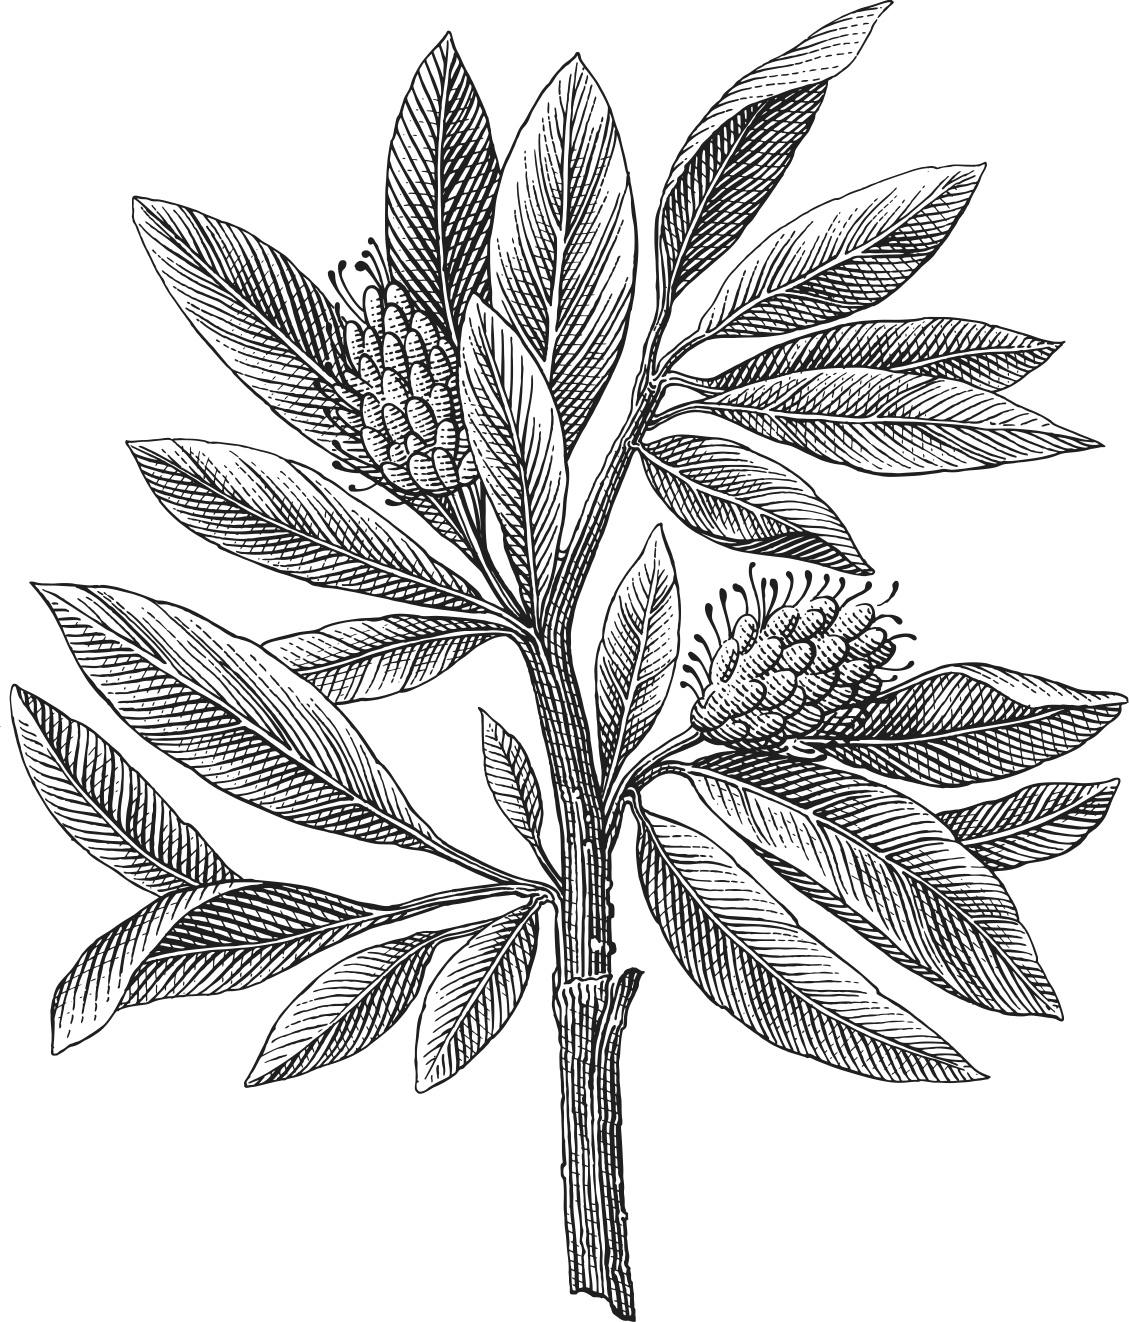
\includegraphics[keepaspectratio,scale=0.65]{lnu_etch.png} % Bakgrundsbild
    }
}
\newcommand\BackgroundPicLogo{
    \put(15,700){
    
\includegraphics[keepaspectratio,scale=0.10]{logo.png} % Logga i vänstra hörnet
    }
}

\newcommand{\horrule}[1]{\rule{\linewidth}{#1}} % Skapa hortisontell linje

\title{	\vspace{-10cm}
    \normalfont \normalsize
    \textsc{Linnéuniversitetet} \\ [25pt] % Universitetes namn
    \horrule{0.5pt} \\[0.4cm] % Tunn linje högst upp
    \huge Laboration 4\\ % Arbetes titel
	\large \textcolor{gray}{1DV020 -- Serveradministraion}
    \horrule{0.5pt} \\[0.4cm] % Tunn linje längst ner
}

% \author{Jacob Lindehoff} % Författarnas namn

\date{\normalsize\today} % Dagens datum

\begin{document}
\AddToShipoutPicture*{\BackgroundPic} % Lägger in backgrundsbild på första sidan
\AddToShipoutPicture*{\BackgroundPicLogo}
\maketitle % Skriv ut titeln
\noindent % Tabba inte in på första meningen

%------------------------------------------------
%	Introduction
%------------------------------------------------
\section{Introduction}

For this module we will work with Active Directory and look at some of the concepts herein. After installing the A.D D.S role we start of by implementing an AGDLP strategy under certain parameters - the exact structure and naming convention will be up to you.

We will then setup group policies on these and assure that we have a proper delegation of control. 

%------------------------------------------------
%	Deadline
%------------------------------------------------
\section{Deadline}
There is only one lab session connected to this module. It is of course okay to present on the following lab.

\paragraph{Accounting} You will show your work and demonstrate your progress at any
of these lab session, prepare a small document with an overview of your configuration/setup if needed for overview.

\paragraph{Note:} To test the environment I will be using the program \textbf{smbclient} from your internal server so make sure that this is installed there. I will also make changes to your groups/add other groups to make sure that the AGDLP is working.


\pagebreak
%------------------------------------------------
%	Uppgift
%------------------------------------------------
\section{Assignment}
The following fours sections with subtasks are the assignment:

\subsection{A.D DS Installation}
Install the Active Directory Domain Services and promote the Windows server to a domain controller.

To be able to have the A.D working properly we need to either delegate the zone corp.mycompany.lab ,so that the linux server instead act as a slave for this zone. Or you can setup a new DNS with forwarders and disable the corp.mycompany.lab on the linux server. This is also a valid workaround. Don't forget to change the DHCP settings.

\subsection{A G/U DLP}
Adopt a AGDLP strategy for the environment specified in the Work Environment, add the users, and groups necessary to accomplish this. You then apply the AGDLP solution on your shares.

\subsection{Join Domain}
Make your internal client(win 8.1 Bus) join the A.D Domain. It should be visible under the computers tab in your A.D structure when you have joined.

(If you run into problems during this phase and gets stuck there. A temporary workaround is to: Follow the “Grant members the right to logon locally” guide to enable logon with local users. This is as said only a temporary solution. But you could confirm that delegation and group policies are working.)

\subsection{Delegation}
Make sure that the following delegations are in effect and make sure you use and AGDLP strategy for this too.
\paragraph{Human Resources:}
\begin{itemize}
	\item Should be able to read user information on all sectors.
\end{itemize}

\paragraph{Call Center Manager:}
\begin{itemize}
	\item Should be able to add, modify and delete regular Callcenter users, but not managers.
	\item Should be able to add, modify and delete regular IT Support users.
\end{itemize}

\paragraph{IT Support:}
Not the same as administrators!
\begin{itemize}
	\item Should be able to add, modify, delete and reset password for Callcenter employees, but not Call Center managers.
	\item Should be able to add, modify and delete regular and reset password for Human resources users.
\end{itemize}

\subsection{Group Policies}
Apply group policies. Try at least 4 group policies and confirm that they are working and affecting only the users in the Call Center OU.
Apply a group policy that only affects the computers of your domain.
Confirm the policies are taking effect.

\subsection{Roaming profiles}
Create a roaming profile for at least one user.

\section{Requirements}
The AGDLP strategy should be working.

If you wish to continue using your current DNS solution you can modify the corp.mycompany.lab zone to act as a slave in your bind configuration and specify the the windows computer as the master for that domain. This of course requires the windows server to be set as  authoritative over that domain.

It should look something like this:
\begin{lstlisting}[style=BashInputStyle]
zone "corp.mycompany.lab" {
    	type slave;
    	masters {<ip of windows server>};
}
\end{lstlisting}
\section{Work Enviroment}
We will assume that the primary role of the company is a call center. We will also assume that we have a decent amount of employees ~50(but for the lab we don’t need to set up all of them!)
\subsection{Sections Layout}
In the environment there should exist the following sections, with employees:
\begin{itemize}
	\item IT Support
	\begin{itemize}
		\item Pelle
	\end{itemize}
\end{itemize}
\begin{itemize}
	\item Human Resources
	\begin{itemize}
		\item Stina
		\item John
	\end{itemize}
\end{itemize}
\begin{itemize}
	\item Call Center
	\begin{itemize}
		\item Manager	
		\begin{itemize}
			\item Johan
		\end{itemize}
		
		\item Employees	
		\begin{itemize}
			\item Marcus
			\item Calina
		\end{itemize}
	\end{itemize}
\end{itemize}

\subsection{Resources}
The following resources should be shared according to your AGDLP solution:
\paragraph{Shares:}
\begin{itemize}
	\item Quick:
	\begin{itemize}
		\item IT Support have full control
		\item Call Center Manager have read and modify Access
		\item  Call Center Employees have read access
		\item  Human resources have read access.
	\end{itemize}
	\item Mirror:
	\begin{itemize}
		\item Call Center manager have full control
		\item  Call Center Employees have Read Access.
		\item  IT support have full control.
	\end{itemize}
\end{itemize}
		
\end{document}
